\documentclass[9pt]{beamer}
\usepackage[utf8]{inputenc}
\usepackage{adjustbox}
\usepackage{amsmath,amssymb,amsthm}
\usepackage{cancel}
\usepackage{float}
\usepackage{mathtools}
\usepackage{tcolorbox}
\usepackage{texdraw}
\usepackage{tikz}
\usepackage{tikz-cd}
\usepackage{todonotes}
\usepackage{blkarray}
\usepackage{multirow}

\renewcommand{\arraystretch}{2}

\tikzset{
commutative diagrams/.cd,
arrow style=tikz,
diagrams={>=latex}}

\usetheme{Warsaw}

\makeatletter
\setbeamertemplate{footline}
{
    \leavevmode%
    \hbox{%
    \begin{beamercolorbox}[wd=.5\paperwidth,ht=3.5ex,dp=2ex,center]{title in head/foot}%
        \usebeamerfont{name in head/foot}{\footnotesize Recovering Matroids}
    \end{beamercolorbox}%
    \begin{beamercolorbox}[wd=.5\paperwidth,ht=3.5ex,dp=2ex,center]{date in head/foot}%
        \usebeamerfont{name in head/foot}{\footnotesize \insertauthor{}}
    \end{beamercolorbox}}%
    \vskip0pt%
}
\makeatother

\usetikzlibrary{arrows.meta}

\def\calM{\mathcal M}
\def\calC{\mathcal C}
\def\calI{\mathcal I}
\def\calD{\mathcal D}
\def\calB{\mathcal B}
\def\calF{\mathcal F}
\def\calN{\mathcal N}
\def\calP{\mathcal P}
\def\calS{\mathcal S}
\def\calV{\mathcal V}
\def\Z{\mathbb Z}
\def\Q{\mathbb Q}

\title{Constructive Torelli Theorem for Regular Matroids}
\author{Alec Elhindi}
\institute{University of Sydney}
\date{Joint Meeting of the New Zealand, Australian and American Mathematical Societies -- 11th December 2024}

\usepackage{graphicx}
\graphicspath{{./images/}}

\newcounter{definition}

\renewcommand{\definition}[1]{\vspace{6pt}\textbf{Definition~\refstepcounter{definition}\thedefinition}: #1\vspace{6pt}}

\newcounter{conjecture}

\newcommand{\conjecture}[1]{\vspace{6pt}\textbf{Conjecture~\refstepcounter{conjecture}\theconjecture}: #1\vspace{6pt}}

\renewcommand{\theorem}[1]{\vspace{6pt}\textbf{Theorem}: #1\vspace{6pt}}

\renewcommand{\corollary}[1]{\vspace{6pt}\textbf{Corollary}: \textit{#1}\vspace{6pt}}

\newcounter{proposition}

\newcommand{\proposition}[1]{\textbf{Proposition}: #1}

\renewcommand{\lemma}[1]{\textbf{Lemma}: #1}

\renewcommand{\example}[1]{\textbf{Example}: #1}

\renewcommand{\proof}[1]{\textbf{Proof}: #1}

\newcommand{\notation}[1]{\textbf{Notation}: #1}

\renewcommand{\qedsymbol}{$\blacksquare$}

\makeatletter
\newcommand{\vast}{\bBigg@{4}}
\newcommand{\Vast}{\bBigg@{5}}
\makeatother

\definecolor{electricpurple}{rgb}{0.75, 0.0, 1.0}

\newcommand{\red}[1]{{\color{red} #1}}
\newcommand{\blue}[1]{{\color{blue} #1}}
\newcommand{\orange}[1]{{\color{orange} #1}}
\newcommand{\purple}[1]{{\color{electricpurple} #1}}

\makeatletter
\let\save@measuring@true\measuring@true
\def\measuring@true{%
  \save@measuring@true
  \def\beamer@sortzero##1{\beamer@ifnextcharospec{\beamer@sortzeroread{##1}}{}}%
  \def\beamer@sortzeroread##1<##2>{}%
  \def\beamer@finalnospec{}%
}
\makeatother

\usetikzlibrary{decorations.markings}

\usetikzlibrary{intersections}

\tikzset{->-/.style={decoration={
    markings,
    mark=at position .5 with {\arrow{>}}},postaction={decorate}}}

\tikzset{-->-/.style={decoration={
    markings,
    mark=at position .75 with {\arrow{>}}},postaction={decorate}}}

\tikzset{->--/.style={decoration={
    markings,
    mark=at position .25 with {\arrow{>}}},postaction={decorate}}}

\tikzcdset{scale cd/.style={every label/.append style={scale=#1},
    cells={nodes={scale=#1}}}}

\DeclarePairedDelimiter\abs{\lvert}{\rvert}

\DeclarePairedDelimiter\norm{\lVert}{\rVert}

\DeclarePairedDelimiter\iprod{\langle}{\rangle}

\DeclareMathOperator{\Short}{Short}

\DeclareMathOperator{\Char}{Char}

\begin{document}

    \begin{frame}

        \titlepage

    \end{frame}

    \begin{frame}{The Lattice of Integer Flows -- Graphs}

        Considering $\Z^E$ to be the free abelian group spanned by $E(G)$, the \textbf{lattice of integer flows} of a graph is the abelian subgroup of $\Z^E$ spanned by cycles, equipped with the Euclidean inner product.

        \pause

        \vspace{12pt}
        
        Any cycle basis is then a basis of the lattice of integer flows.

        \pause

        \vspace{12pt}

        The \textbf{discrete Torelli theorem} for a certain class of objects states that their lattices of integer flows are isomorphic iff the objects are.

        \pause

        \vspace{12pt}

        \begin{center}

            \begin{tabular}{c|c|c}
                $\frac{\text{Graphs}}{\text{2-isomorphism}}$ & $\frac{\text{Laplacians}}{\text{unimodular congruence}}$ & Watkins (1990, 1994)\pause\\
                \hline
                $\frac{\text{Graphs}}{\text{2-isomorphism}}$ & $\frac{\text{Albanese torus}}{\text{isomorphism}}$ & \multirow{2}{*}{Caporaso and Viviani (2010)}\\
                $\frac{\text{Compact tropical curves}}{\text{tropical equivalence}}$ & $\frac{\text{Jacobian varieties}}{\text{isomorphism}}$ & \pause\\
                \hline
                $\frac{\text{Regular matroids/coloops}}{\text{isomorphism}}$ & $\frac{\text{Lattice of integer flows}}{\text{isomorphism}}$ & Su and Wagner (2010)
            \end{tabular}

        \end{center}
        
    \end{frame}

    \begin{frame}{The Lattice of Integer Flows -- Graphs}

        \begin{center}
        
            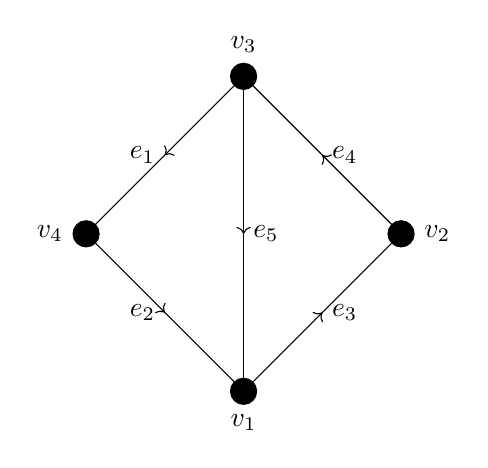
\begin{tikzpicture}
            
                \node[shape=circle, draw=black, fill=black, label=below:$v_1$] (A) at (0,0) {};
                \node[shape=circle, draw=black, fill=black, label=right:$v_2$] (B) at (2,2) {};
                \node[shape=circle, draw=black, fill=black, label=above:$v_3$] (C) at (0,4) {};
                \node[shape=circle, draw=black, fill=black, label=left:$v_4$] (D) at (-2,2) {};
            
                \draw[->-] (C) -- (D) node[midway, left] {$e_1$};
                \draw[->-] (D) -- (A) node[midway, left] {$e_2$};
                \draw[->-] (A) -- (B) node[midway, right] {$e_3$};
                \draw[->-] (B) -- (C) node[midway, right] {$e_4$};
                \draw[->-] (C) -- (A) node[midway, right] {$e_5$};
        
            \end{tikzpicture}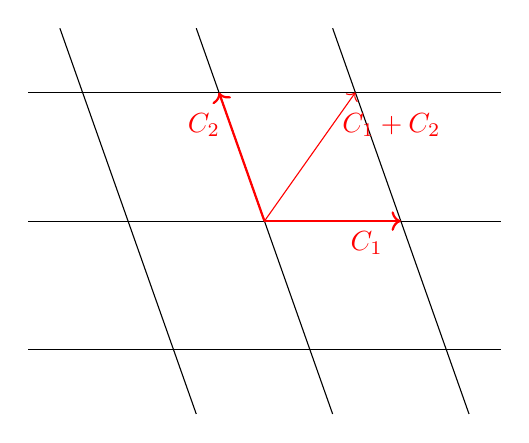
\begin{tikzpicture}

                \draw (-3,-1.63299316) -- (3,-1.63299316);
                \draw (-3,0) -- (3,0);
                \draw (-3,1.63299316) -- (3,1.63299316);
                \draw (-0.57735027*1.5-1.73205081,1.63299316*1.5) -- (0.57735027*1.5-1.73205081,-1.63299316*1.5);
                \draw (-0.57735027*1.5,1.63299316*1.5) -- (0.57735027*1.5,-1.63299316*1.5);
                \draw (-0.57735027*1.5+1.73205081,1.63299316*1.5) -- (0.57735027*1.5+1.73205081,-1.63299316*1.5);

                \draw[->, thick, red] (0,0) -- (1.73205081,0) node[near end, below, red] {$C_1$};
                \draw[->, thick, red] (0,0) -- (-0.57735027,1.63299316) node[near end, left, red] {$C_2$};
                \draw[->, red] (0,0) -- (-0.57735027+1.73205081,1.63299316) node[near end, right, red] {$C_1+C_2$};

            \end{tikzpicture}

            \[C_1=+e_1+e_2-e_5, \quad C_2=+e_3+e_4+e_5, \quad C_1+C_2=+e_1+e_2+e_3+e_4.\]
        
        \end{center}
        
    \end{frame}

    \begin{frame}{The Lattice of Integer Flows -- Regular Matroids}
        
        Given a regular matroid $\calM$ with representing matrix $M$, the lattice of integer flows is

        \[\calF(\calM)=\ker(M)\cap\Z^E.\]
        This coincides for the signed incidence matrix of a graph -- the natural representing matrix for a graphical matroid.

    \end{frame}

    \begin{frame}{Recovering $\calM$}

        \theorem{[Su--Wagner] Let $\calM$ and $\calN$ be matroids of cogirth $\geq2$.
        Then $\calF(\calM)\cong\calF(\calN)$ if and only if $\calM\cong\calN$.}

        \pause

        \vspace{12pt}

        We provide a constructive algorithm for recovering the matroid -- a \textit{constructive Torelli theorem}.
        The first step is the following strengthening of the discrete Torelli theorem for matroids.

        \pause

        \vspace{12pt}

        \proposition{[Dancso--E.--Garoufalidis] An isomorphism of lattices $\varphi:\calF(\calM)\rightarrow\calF(\calN)$ lifts to an isomorphism $\Phi:\Z^{E(\calM)}\rightarrow\Z^{E(\calN)}$.}
        
        \pause

        \vspace{12pt}

        Assume all matroids are of cogirth $\geq2$.
        Note that a matroid has cogirth $\geq2$ if and only if it can be oriented totally cyclically.

    \end{frame}

    \begin{frame}{Voronoi Cells}

        Recovering $\calM$ comes down to: detecting which elements in $\calF(\calM)$ are circuit elements, determining the base set of $\calM$, and determining which elements are in each circuit.

        \pause

        \vspace{12pt}

        The key to the recovery is through analysing a polytope in the lattice, called the Voronoi cell.

        \pause

        \vspace{12pt}

        The \textbf{Voronoi cell} $\calV(\Lambda)$ of a lattice $\Lambda$ is the collection of points in space (i.e. in $\Lambda\otimes\mathbb{R}$) closer to the origin than any other lattice point in $\Lambda$.

    \end{frame}

    \begin{frame}{Voronoi Cells}

        \begin{center}
        
            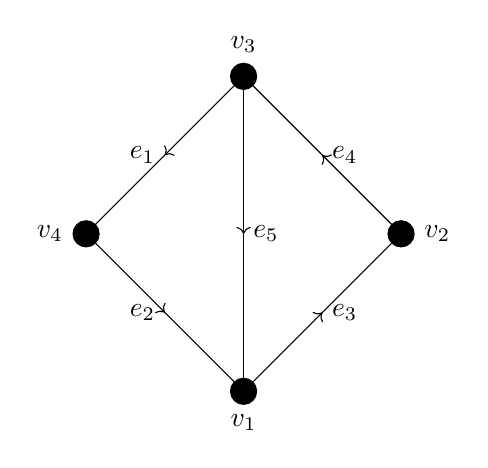
\begin{tikzpicture}
            
                \node[shape=circle, draw=black, fill=black, label=below:$v_1$] (A) at (0,0) {};
                \node[shape=circle, draw=black, fill=black, label=right:$v_2$] (B) at (2,2) {};
                \node[shape=circle, draw=black, fill=black, label=above:$v_3$] (C) at (0,4) {};
                \node[shape=circle, draw=black, fill=black, label=left:$v_4$] (D) at (-2,2) {};
            
                \draw[->-] (C) -- (D) node[midway, left] {$e_1$};
                \draw[->-] (D) -- (A) node[midway, left] {$e_2$};
                \draw[->-] (A) -- (B) node[midway, right] {$e_3$};
                \draw[->-] (B) -- (C) node[midway, right] {$e_4$};
                \draw[->-] (C) -- (A) node[midway, right] {$e_5$};
        
            \end{tikzpicture}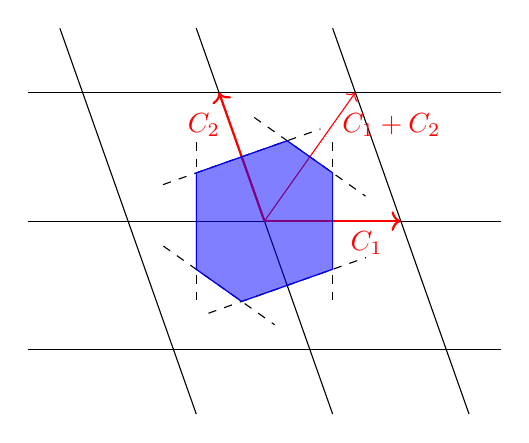
\begin{tikzpicture}

                %sqrt3=1.73205081
                %1/sqrt3=0.57735027
                %2sqrt2/sqrt3=1.63299316
                %1/2sqrt2=0.35355339
                %sqrt2=1.41421356

                \draw (-3,-1.63299316) -- (3,-1.63299316);
                \draw (-3,0) -- (3,0);
                \draw (-3,1.63299316) -- (3,1.63299316);
                \draw (-0.57735027*1.5-1.73205081,1.63299316*1.5) -- (0.57735027*1.5-1.73205081,-1.63299316*1.5);
                \draw (-0.57735027*1.5,1.63299316*1.5) -- (0.57735027*1.5,-1.63299316*1.5);
                \draw (-0.57735027*1.5+1.73205081,1.63299316*1.5) -- (0.57735027*1.5+1.73205081,-1.63299316*1.5);

                \draw[dashed, name path=line 1] (-1.73205081/2,1) -- (-1.73205081/2,-1);
                \draw[dashed, name path=line 2] (1.73205081/2,1) -- (1.73205081/2,-1);
                \draw[dashed, name path=line 3] (-0.57735027/2-1,1.63299316/2-0.35355339) -- (-0.57735027/2+1,1.63299316/2+0.35355339);
                \draw[dashed, name path=line 4] (0.57735027/2-1,-1.63299316/2-0.35355339) -- (0.57735027/2+1,-1.63299316/2+0.35355339);
                \draw[dashed, name path=line 5] (-0.57735027/2+1.73205081/2-1.41421356*1/2,1.63299316/2+1/2) -- (-0.57735027/2+1.73205081/2+1.41421356*1/2,1.63299316/2-1/2);
                \draw[dashed, name path=line 6] (0.57735027/2-1.73205081/2-1.41421356*1/2,-1.63299316/2+1/2) -- (0.57735027/2-1.73205081/2+1.41421356*1/2,-1.63299316/2-1/2);

                \draw[->, thick, red] (0,0) -- (1.73205081,0) node[near end, below, red] {$C_1$};
                \draw[->, thick, red] (0,0) -- (-0.57735027,1.63299316) node[near end, left, red] {$C_2$};
                \draw[->, red] (0,0) -- (-0.57735027+1.73205081,1.63299316) node[near end, right, red] {$C_1+C_2$};

                \path[name intersections={of=line 1 and line 3, by=A}];
                \path[name intersections={of=line 1 and line 6, by=B}];
                \path[name intersections={of=line 4 and line 6, by=C}];
                \path[name intersections={of=line 2 and line 4, by=D}];
                \path[name intersections={of=line 2 and line 5, by=E}];
                \path[name intersections={of=line 3 and line 5, by=F}];

                \draw[fill=blue, opacity=0.5] (A) -- (B) -- (C) -- (D) -- (E) -- (F) -- (A);

                \def\points{(A), (B), (C), (D), (E), (F), (A)}
                
                \foreach \p [count=\i, remember=\p as \lastp] in \points{
                    \ifnum\i>1\relax
                    %\node[shape=circle, scale=0.2, draw=blue, fill=blue]  at \p {};
                    \path[draw=blue, fill=blue] \lastp -- \p;
                    \fi
                }

            \end{tikzpicture}

            \[C_1=+e_1+e_2-e_5, \quad C_2=+e_3+e_4+e_5, \quad C_1+C_2=+e_1+e_2+e_3+e_4.\]
        
        \end{center}
        
    \end{frame}

    \begin{frame}{Amini-Dancso-Lim Theorem}

        Faces of the Voronoi cell form a poset $\calF\calP(\calF(\calM))$ with inclusion given by dimension.

        \vspace{12pt}

        Orientations on $\calM$ and its submatroids which are totally cyclic form a poset $\calS\calC(\calM)$ where $(\calN', \omega_{\calN'})\leq(\calN, \omega_\calN)$ if and only if $\calN$ is a submatroid of $\calN'$ and $\omega_{\calN'}$ restricted to $\calN$ is $\omega_\calN$.

        \pause

        \vspace{12pt}

        \theorem{[Amini-Dancso-Lim] For a finite regular matroid $\calM$, $\calF\calP(\calF(\calM))\cong\calS\calC(\calM)$ as graded posets.}
        
    \end{frame}

    \begin{frame}{Amini-Dancso-Lim Theorem}

        \example{Codimension one faces of the Voronoi cell correspond to circuits in $\calM$.
        Edges of the Voronoi cell correspond to maximal totally cyclical submatroids of $\calM$.}

        \pause

        \vspace{12pt}

        The parallel faces of the Voronoi cell correspond to the different totally cyclic orientations of the same underlying matroid, so denote the \textbf{equivalence class of faces that are parallel to $F$} by $[F]$.

        \vspace{12pt}

        For a subset $A\subseteq E(\calM)$ we denote $[F_A]$ to be the face(s) which corresponds to $\calM\setminus A$ (provided it is totally cyclically orientable).
        
    \end{frame}

    \begin{frame}{Reconstruction for Cogirth $\geq3$ Matroids}

        For all $e\in E(\calM)$, the submatroid $\calM\setminus\{e\}$ has cogirth $\geq2$, so can be totally cyclically oriented.

        \vspace{12pt}

        \theorem{[Dancso--E.--Garoufalidis] For matroids of cogirth $\geq3$:}

        \pause

        \vspace{-6pt}
        
        \begin{enumerate}
            \item $e\in E(\calM)\xleftrightarrow{1:1}[F_{\{e\}}]\;\text{edges}$,\pause
            \item $C\in\calC(\calM)\xleftrightarrow{1:1}[F_C]$ codimension one faces,\pause
            \item $e\in C\xLeftrightarrow{\textcolor{white}{::}} [F_{\{e\}}]\not\leq [F_C]$.\pause
        \end{enumerate}

        \vspace{12pt}

        For general matroids of cogirth $\geq2$ steps (2) and (3) remain the same, but step (1) requires much more work, as maximal totally cyclic submatroids may be of the form $\calM\setminus S$ for (possibly different sized) $\abs*{S}>1$.
        
    \end{frame}

    \begin{frame}{2-Cut Blocks}

        They turn out to be what we call \textbf{2-cut blocks}.
        These are the equivalence classes of the equivalence relation $e\sim f$ if and only if $e=f$ or $\{e, f\}$ is a cocircuit.

        \pause

        \vspace{12pt}

        \begin{figure}[htbp]

            \begin{center}
            
                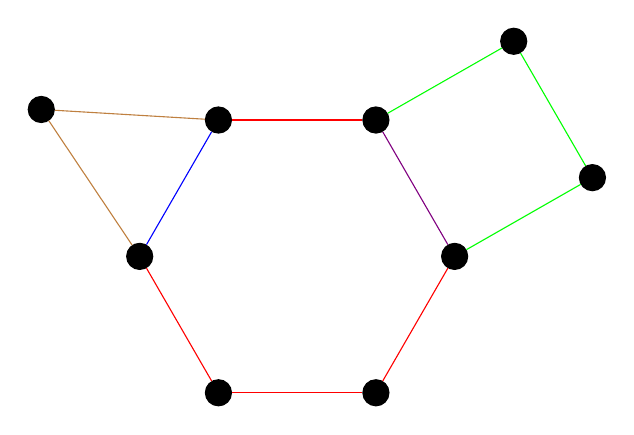
\begin{tikzpicture}
        
                    \node[shape=circle, draw=black, fill=black] (A) at (60:2) {};
                    \node[shape=circle, draw=black, fill=black] (B) at (120:2) {};
                    \node[shape=circle, draw=black, fill=black] (C) at (180:2) {};
                    \node[shape=circle, draw=black, fill=black] (D) at (240:2) {};
                    \node[shape=circle, draw=black, fill=black] (E) at (300:2) {};
                    \node[shape=circle, draw=black, fill=black] (F) at (360:2) {};
                    \node[shape=circle, draw=black, fill=black] (G) at (2.75, 2.73205) {};
                    \node[shape=circle, draw=black, fill=black] (H) at (3.75, 1) {};
                    \node[shape=circle, draw=black, fill=black] (I) at (-3.25, 1.866025) {};
                
                    \draw[red] (A) -- (B);
                    \draw[blue] (B) -- (C);
                    \draw[red] (C) -- (D);
                    \draw[red] (D) -- (E);
                    \draw[red] (E) -- (F);
                    \draw[violet] (F) -- (A);
                    \draw[green] (A) -- (G);
                    \draw[green] (F) -- (H);
                    \draw[green] (G) -- (H);
                    \draw[brown] (B) -- (I);
                    \draw[brown] (C) -- (I);
            
                \end{tikzpicture}
            
            \end{center}
        
        \end{figure}

    \end{frame}

    \begin{frame}{2-Cut Blocks}

        \proposition{[Dancso--E.--Garoufalidis] Given a circuit $C$ and a 2-cut block $S$, either $S\cap C=\emptyset$ or $S\subseteq C$.}

        \pause

        \vspace{12pt}

        So we can write a circuit as a disjoint union of 2-cut blocks.

        \pause

        \vspace{12pt}

        \proposition{[Dancso--E.--Garoufalidis] $\calM\setminus S$ is a maximal submatroid of $\calM$ with cogirth $\geq2$ if and only if $S$ is a 2-cut block.}

        \pause

        \vspace{12pt}
        
        For a parallel class of edges $[\epsilon]$, let $S_{[\epsilon]}$ be the corresponding 2-cut block.
        Then with Amini's theorem we can write,

        \[C=\bigcup_{[\epsilon]\not\in [F_C]} S_{[\epsilon]}.\]

        \pause

        \vspace{12pt}

        We need to detect the sizes of $S_{[\epsilon]}$ from the sizes of circuits.
        This can be done using the pairwise inner product of circuit basis elements, but we want to choose a clever basis.
        
    \end{frame}

    \begin{frame}{Compatibly Oriented Bases}

        For any circuits $C_i, C_j$ and their corresponding faces $F_{C_i}, F_{C_j}$, there are three possible options:\pause

        \begin{enumerate}
            \item The orientations of $C_i$ and $C_j$ are compatible.
            This is the case if and only if $F_{C_i}$ and $F_{C_j}$ intersect.\pause
            \item The orientations of $C_i$ and $-C_j$ are compatible.
            This is the case if and only if $F_{C_i}$ and $F_{-C_j}$ intersect.\pause
            \item Neither of the above is true, that is, $C_i$ and $C_j$ cannot be compatibly oriented.
            This is the case if and only if the faces $\{F_{C_i}, F_{C_j}, F_{-C_i}, F_{-C_j}\}$ are pairwise disjoint.\pause
        \end{enumerate}

        Amini's theorem tells us that vertices correspond to totally cyclic orientations.
        Take any vertex, then the codimension one faces that intersect at that vertex form a compatibly oriented basis.
        
    \end{frame}

    \begin{frame}{Reconstruction for Cogirth $2$ Matroids}

        \theorem{[Dancso--E.--Garoufalidis] For matroids of cogirth $2$:}

        \pause

        \vspace{-6pt}
        
        \begin{enumerate}
            \item Create a circuit basis $B$ such that $\abs*{\iprod*{C_i, C_j}}=\abs*{C_i\cap C_j}$ for all $C_i, C_j\in B$.\pause
            \item Find the parallel classes $[\epsilon]$ of the Voronoi cell and identify which edges participate in $[F_C]$ for each $C\in B$.\pause
            \item For each basis circuit $C_i, i=1, \dots, r$, write the equation

            \[\sum_{[\epsilon]\not\in [F_{C_i}]} \abs*{S_{[\epsilon]}}=\iprod*{C_i, C_i},\]
            and for each pair of basis circuits $\{\{C_i, C_j\}, i, j=1, \dots, r, i\neq j\}$ write the equation
            
            \[\sum_{[\epsilon]\not\in [F_{C_i}], [F_{C_j}]} \abs*{S_{[\epsilon]}}=\abs*{\iprod*{C_i, C_j}}.\]\pause
            \item Find the unique positive integer solution $\{\abs*{S_{[\epsilon]}}\}$.\pause
            \item $E(\calM)$ is the disjoint union of the sets $\{S_{[\epsilon]}\}$.\pause
            \item Again, the element $e\in S_{[\epsilon]}$ belongs to a circuit $C$ if and only if no member of the corresponding edge parallel class $[\epsilon]$ belongs to the face $[F_C]$.
        \end{enumerate}
        
    \end{frame}

    \begin{frame}{Uniqueness}

        \proposition{[Dancso--E.--Garoufalidis] There is a unique positive integer solution $\{\abs*{S_{[\epsilon]}}\}$ to the system of equations in (3).}

        \pause

        \vspace{12pt}

        \proof{\begin{itemize}
            \item There is some solution given by the (oriented) matroid $\calM$ which exists by definition, call this $\{m_{[\epsilon]}\}$.\pause
            \item Suppose there exists another (oriented) matroid $\calN$ with solution $\{n_{[\epsilon]}\}$.\pause
            \item Contractions and subdivisions in a 2-cut block do not change circuits.\pause
            \item Apply contractions and subdivisions to $\calM$ until these integer solutions match.\pause
            \item The circuits are in correspondence, which is an isomorphism of lattices of integer flows, thus lifts to an isomorphism of euclidean lattices, inducing a matroid isomorphism of $\calM$.
        \end{itemize}}

        \hspace*{\fill}\qedsymbol
        
    \end{frame}

    \begin{frame}{Reconstructing}

        \begin{minipage}{0.4\textwidth}

            \begin{figure}[htbp]
            
                \begin{center}
            
                    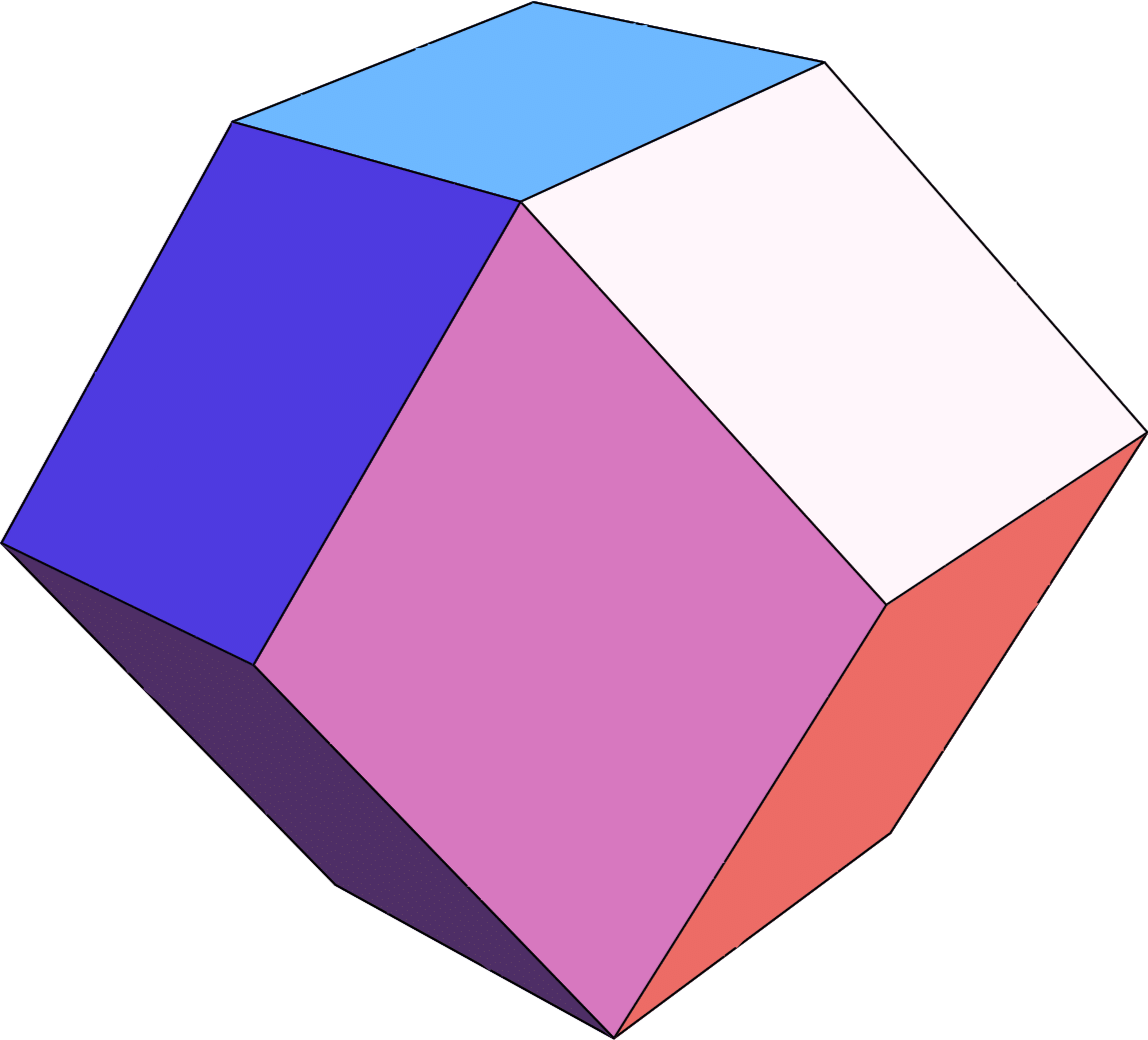
\includegraphics[height=3cm]{RhombicDodecahedron.png}
                    
                \end{center}
                
            \end{figure}

            \renewcommand{\arraystretch}{1.25}

            \[\begin{blockarray}{cccc}
                & C_1 & C_2 & C_3\\
                \begin{block}{c(ccc)}
                    C_1 & 3 & 1 & 2\\
                    C_2 & 1 & 3 & 0\\
                    C_3 & 2 & 0 & 4\\
                \end{block}
            \end{blockarray}\]
            
        \end{minipage}\resizebox{0.1\textwidth}{!}{$\rightarrow$}\begin{minipage}{0.5\textwidth}

            \begin{figure}[htbp]
            
                \begin{center}
    
                    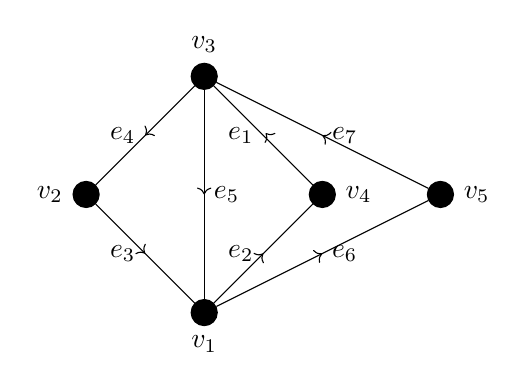
\begin{tikzpicture}[scale=0.75]
                    
                        \node[shape=circle, draw=black, fill=black, label=below:$v_1$] (A) at (0,0) {};
                        \node[shape=circle, draw=black, fill=black, label=left:$v_2$] (B) at (-2,2) {};
                        \node[shape=circle, draw=black, fill=black, label=above:$v_3$] (C) at (0,4) {};
                        \node[shape=circle, draw=black, fill=black, label=right:$v_4$] (D) at (2,2) {};
                        \node[shape=circle, draw=black, fill=black, label=right:$v_5$] (E) at (4,2) {};
                    
                        \draw[->-] (D) -- (C) node[midway, left] {$e_1$};
                        \draw[->-] (A) -- (D) node[midway, left] {$e_2$};
                        \draw[->-] (B) -- (A) node[midway, left] {$e_3$};
                        \draw[->-] (C) -- (B) node[midway, left] {$e_4$};
                        \draw[->-] (C) -- (A) node[midway, right] {$e_5$};
                        \draw[->-] (A) -- (E) node[midway, right] {$e_6$};
                        \draw[->-] (E) -- (C) node[midway, right] {$e_7$};
                
                    \end{tikzpicture}
                
                \end{center}
            
            \end{figure}

            \vspace{-24pt}

            \begin{align*}
                C_1&=+e_1+e_2+e_5,\\
                C_2&=+e_5+e_6+e_7,\\
                C_3&=+e_1+e_2+e_3+e_4.
            \end{align*}

        \end{minipage}
        
    \end{frame}

    \begin{frame}{Lifting Isomorphisms}

        \proposition{[Dancso--E.--Garoufalidis] An isomorphism of lattices $\varphi:\calF(\calM)\rightarrow\calF(\calN)$ lifts to an isomorphism $\Phi:\Z^{E(\calM)}\rightarrow\Z^{E(\calN)}$.}

        \pause

        \vspace{12pt}

        \proof{\begin{enumerate}
            \item \lemma{[Dancso--E.--Garoufalidis] A matroid of cogirth $\geq2$ can be oriented totally cyclically and oriented s.t. it admits a positive circuit basis.}\pause
            \item Automorphisms of $\calF(\calM)$ lift -- Greene's rigid embedding theorem and (1).\pause
            \item
        \end{enumerate}

        \begin{center}

            \begin{tikzcd}[row sep=large,column sep=huge,ampersand replacement=\&]
                \textcolor{white}{\Z^{E(\calM)}}
                    \arrow[white]{r}[white]{\Psi}
                \& \Z^{E(\calN)}
                    
                \& \Z^{E(\calM)}
                    \arrow[dashed]{l}[swap]{\Phi}
                    \arrow[bend right, white]{ll}[swap, white]{F}
                    \\
                \textcolor{white}{\calF(\calM)}
                    \arrow[white]{r}[swap, white]{\psi}
                    \arrow[hookrightarrow, white]{u}[white]{}
                \& \calF(\calN)
                    \arrow[hookrightarrow, white]{u}[swap, white]{}
                \& \calF(\calM)
                    \arrow{l}{\varphi}
                    \arrow[hookrightarrow, white]{u}[swap, white]{}
                    \arrow[bend left, white]{ll}[white]{\psi^{-1}\circ\varphi}

            \end{tikzcd}
            
        \end{center}

        \textcolor{white}{\hspace*{\fill}\qedsymbol}}
        
    \end{frame}

    \begin{frame}{Lifting Isomorphisms}

        \proposition{[Dancso--E.--Garoufalidis] An isomorphism of lattices $\varphi:\calF(\calM)\rightarrow\calF(\calN)$ lifts to an isomorphism $\Phi:\Z^{E(\calM)}\rightarrow\Z^{E(\calN)}$.}

        \vspace{12pt}

        \proof{\begin{enumerate}
            \item \lemma{[Dancso--E.--Garoufalidis] A matroid of cogirth $\geq2$ can be oriented totally cyclically and oriented s.t. it admits a positive circuit basis.}
            \item Automorphisms of $\calF(\calM)$ lift -- Greene's rigid embedding theorem and (1).
            \item
        \end{enumerate}

        \begin{center}

            \begin{tikzcd}[row sep=large,column sep=huge,ampersand replacement=\&]
                \Z^{E(\calM)}
                    \arrow{r}{\Psi}
                \& \Z^{E(\calN)}
                    
                \& \Z^{E(\calM)}
                    \arrow[dashed]{l}[swap]{\Phi}
                    \arrow[bend right, white]{ll}[swap, white]{F}
                    \\
                \textcolor{white}{\calF(\calM)}
                    \arrow[white]{r}[swap, white]{\psi}
                    \arrow[hookrightarrow, white]{u}[white]{}
                \& \calF(\calN)
                    \arrow[hookrightarrow, white]{u}[swap, white]{}
                \& \calF(\calM)
                    \arrow{l}{\varphi}
                    \arrow[hookrightarrow, white]{u}[swap, white]{}
                    \arrow[bend left, white]{ll}[white]{\psi^{-1}\circ\varphi}

            \end{tikzcd}
            
        \end{center}

        \textcolor{white}{\hspace*{\fill}\qedsymbol}}
        
    \end{frame}

    \begin{frame}{Lifting Isomorphisms}

        \proposition{[Dancso--E.--Garoufalidis] An isomorphism of lattices $\varphi:\calF(\calM)\rightarrow\calF(\calN)$ lifts to an isomorphism $\Phi:\Z^{E(\calM)}\rightarrow\Z^{E(\calN)}$.}

        \vspace{12pt}

        \proof{\begin{enumerate}
            \item \lemma{[Dancso--E.--Garoufalidis] A matroid of cogirth $\geq2$ can be oriented totally cyclically and oriented s.t. it admits a positive circuit basis.}
            \item Automorphisms of $\calF(\calM)$ lift -- Greene's rigid embedding theorem and (1).
            \item
        \end{enumerate}

        \begin{center}

            \begin{tikzcd}[row sep=large,column sep=huge,ampersand replacement=\&]
                \Z^{E(\calM)}
                    \arrow{r}{\Psi}
                \& \Z^{E(\calN)}
                    
                \& \Z^{E(\calM)}
                    \arrow[dashed]{l}[swap]{\Phi}
                    \arrow[bend right, white]{ll}[swap, white]{F}
                    \\
                \calF(\calM)
                    \arrow{r}[swap]{\psi}
                    \arrow[hookrightarrow, white]{u}[white]{}
                \& \calF(\calN)
                    \arrow[hookrightarrow, white]{u}[swap, white]{}
                \& \calF(\calM)
                    \arrow{l}{\varphi}
                    \arrow[hookrightarrow, white]{u}[swap, white]{}
                    \arrow[bend left, white]{ll}[white]{\psi^{-1}\circ\varphi}
            \end{tikzcd}
            
        \end{center}

        \textcolor{white}{\hspace*{\fill}\qedsymbol}}
        
    \end{frame}

    \begin{frame}{Lifting Isomorphisms}

        \proposition{[Dancso--E.--Garoufalidis] An isomorphism of lattices $\varphi:\calF(\calM)\rightarrow\calF(\calN)$ lifts to an isomorphism $\Phi:\Z^{E(\calM)}\rightarrow\Z^{E(\calN)}$.}

        \vspace{12pt}

        \proof{\begin{enumerate}
            \item \lemma{[Dancso--E.--Garoufalidis] A matroid of cogirth $\geq2$ can be oriented totally cyclically and oriented s.t. it admits a positive circuit basis.}
            \item Automorphisms of $\calF(\calM)$ lift -- Greene's rigid embedding theorem and (1).
            \item
        \end{enumerate}

        \begin{center}

            \begin{tikzcd}[row sep=large,column sep=huge,ampersand replacement=\&]
                \Z^{E(\calM)}
                    \arrow{r}{\Psi}
                \& \Z^{E(\calN)}
                    
                \& \Z^{E(\calM)}
                    \arrow[dashed]{l}[swap]{\Phi}
                    \arrow[bend right, white]{ll}[swap, white]{F}
                    \\
                \calF(\calM)
                    \arrow{r}[swap]{\psi}
                    \arrow[hookrightarrow, white]{u}[white]{}
                \& \calF(\calN)
                    \arrow[hookrightarrow, white]{u}[swap, white]{}
                \& \calF(\calM)
                    \arrow{l}{\varphi}
                    \arrow[hookrightarrow, white]{u}[swap, white]{}
                    \arrow[bend left]{ll}{\psi^{-1}\circ\varphi}
            \end{tikzcd}
            
        \end{center}

        \textcolor{white}{\hspace*{\fill}\qedsymbol}}
        
    \end{frame}

    \begin{frame}{Lifting Isomorphisms}

        \proposition{[Dancso--E.--Garoufalidis] An isomorphism of lattices $\varphi:\calF(\calM)\rightarrow\calF(\calN)$ lifts to an isomorphism $\Phi:\Z^{E(\calM)}\rightarrow\Z^{E(\calN)}$.}

        \vspace{12pt}

        \proof{\begin{enumerate}
            \item \lemma{[Dancso--E.--Garoufalidis] A matroid of cogirth $\geq2$ can be oriented totally cyclically and oriented s.t. it admits a positive circuit basis.}
            \item Automorphisms of $\calF(\calM)$ lift -- Greene's rigid embedding theorem and (1).
            \item
        \end{enumerate}

        \begin{center}

            \begin{tikzcd}[row sep=large,column sep=huge,ampersand replacement=\&]
                \Z^{E(\calM)}
                    \arrow{r}{\Psi}
                \& \Z^{E(\calN)}
                    
                \& \Z^{E(\calM)}
                    \arrow[dashed]{l}[swap]{\Phi}
                    \arrow[bend right]{ll}[swap]{F}
                    \\
                \calF(\calM)
                    \arrow{r}[swap]{\psi}
                    \arrow[hookrightarrow, white]{u}[white]{}
                \& \calF(\calN)
                    \arrow[hookrightarrow, white]{u}[swap, white]{}
                \& \calF(\calM)
                    \arrow{l}{\varphi}
                    \arrow[hookrightarrow, white]{u}[swap, white]{}
                    \arrow[bend left]{ll}{\psi^{-1}\circ\varphi}
            \end{tikzcd}
            
        \end{center}

        \textcolor{white}{\hspace*{\fill}\qedsymbol}}
        
    \end{frame}

    \begin{frame}{Lifting Isomorphisms}

        \proposition{[Dancso--E.--Garoufalidis] An isomorphism of lattices $\varphi:\calF(\calM)\rightarrow\calF(\calN)$ lifts to an isomorphism $\Phi:\Z^{E(\calM)}\rightarrow\Z^{E(\calN)}$.}

        \vspace{12pt}

        \proof{\begin{enumerate}
            \item \lemma{[Dancso--E.--Garoufalidis] A matroid of cogirth $\geq2$ can be oriented totally cyclically and oriented s.t. it admits a positive circuit basis.}
            \item Automorphisms of $\calF(\calM)$ lift -- Greene's rigid embedding theorem and (1).
            \item
        \end{enumerate}

        \begin{center}

            \begin{tikzcd}[row sep=large,column sep=huge,ampersand replacement=\&]
                \Z^{E(\calM)}
                    \arrow[blue]{r}{\Psi}
                \& \Z^{E(\calN)}
                    
                \& \Z^{E(\calM)}
                    \arrow[dashed]{l}[swap]{\textcolor{blue}{\Phi:=\Psi\circ F}}
                    \arrow[bend right, blue]{ll}[swap]{F}
                    \\
                \calF(\calM)
                    \arrow{r}[swap]{\psi}
                    \arrow[hookrightarrow]{u}{}
                \& \calF(\calN)
                    \arrow[hookrightarrow]{u}[swap]{}
                \& \calF(\calM)
                    \arrow{l}{\varphi}
                    \arrow[hookrightarrow]{u}[swap]{}
                    \arrow[bend left]{ll}{\psi^{-1}\circ\varphi}
            \end{tikzcd}
            
        \end{center}

        \hspace*{\fill}\qedsymbol}
        
    \end{frame}
    
\end{document}
